\documentclass[newpage]{homework}
\newcommand{\hwname}{Zooey Nguyen}
\newcommand{\hwemail}{zooeyn@ucla.edu}
\newcommand{\hwclass}{CS 146}
\newcommand{\hwtype}{Homework}
\newcommand{\hwnum}{6}
\begin{document}
\maketitle


\question
Sigmoid form of conditional probability.
\begin{align*}
    P(C_0|x)	&=	\frac{P(x|C_0)P(C_0)}{P(x|C_0)P(C_0)+P(x|C_1)P(C_1)}	\\
    P(C_0|x)	&=	\frac{1}{1+\frac{P(x|C_1)P(C_1)}{P(x|C_0)P(C_0)}}	\\
    P(C_0|x)	&=	\frac{1}{1+\exp{\ln \frac{P(x|C_1)P(C_1)}{P(x|C_0)P(C_0)}}}	\\
    P(C_0|x)	&=	\frac{1}{1+\exp{\ln P(x|C_1)P(C_1) - \ln P(x|C_0)P(C_0) }}	\\
    P(C_0|x)	&=  \frac{1}{1+\exp{-(\ln P(x|C_0)P(C_0) - \ln P(x|C_1)P(C_1))}}    \\
    P(C_0|x)	&=	\boxed{\frac{1}{1+\exp{-a}}}	\\
    a    &= \boxed{\ln \frac{P(x|C_0)P(C_0)}{P(x|C_1)P(C_1)} }  \\
\end{align*}
Linear form of a.
\begin{align*}
    a	&=	\ln \frac{P(x|C_0)P(C_0)}{P(x|C_1)P(C_1)}	\\
    a	&=	(x-\mu_0)^T \Sigma^{-1} (x-\mu_0) P(C_0) - (x-\mu_1)^T \Sigma^{-1} (x-\mu_1) P(C_1)   \\
    a	&=	(x^T-\mu_0^T) \Sigma^{-1} (x-\mu_0) P(C_0) - (x^T-\mu_1^T) \Sigma^{-1} (x-\mu_1) P(C_1)   \\
    a	&=	[x^T\Sigma^{-1}x + \mu_0^T \Sigma^{-1} \mu_0] P(C_0) - [x^T\Sigma^{-1}x + \mu_1^T \Sigma^{-1} \mu_1] P(C_1)   \\
    a	&=	\left[x^T\Sigma^{-1}P(C_0) - x^T\Sigma^{-1}P(C_1)\right] x + \left[\mu_0^T \Sigma^{-1} \mu_0 P(C_0) - \mu_1^T \Sigma^{-1} \mu_1] P(C_1) \right]    \\
    a   &=  \boxed{w^Tx+b}  \\
    w   &=  \left[x^T\Sigma^{-1}P(C_0) - x^T\Sigma^{-1}P(C_1)\right]^T \\
    w   &=  \left[x^T\Sigma^{-1}P(C_0)\right]^T - \left[x^T\Sigma^{-1}P(C_1)\right]^T \\
    w   &=  (P(C_0) \Sigma x - P(C_1) \Sigma x) \\
    w   &=  \boxed{[P(C_0) - P(C_1)]\Sigma x }\\
    b   &=  \boxed{\mu_0^T \Sigma^{-1} \mu_0 P(C_0) - \mu_1^T \Sigma^{-1} \mu_1 P(C_1)}
\end{align*}
Linear form of a with different covariance matrices. Note that this is the exact same as before but we are adding the following term to a.
\begin{align*}
    a	&=	\ln \frac{P(x|C_0)P(C_0)}{P(x|C_1)P(C_1)}	\\
    a	&=	\ln\frac{|\Sigma_1|^{1/2}}{|\Sigma_0|^{1/2}} \left[(x-\mu_0)^T \Sigma_0^{-1} (x-\mu_0) P(C_0) - (x-\mu_1)^T \Sigma_1^{-1} (x-\mu_1) P(C_1)\right]   \\
    a	&=	\ln\frac{|\Sigma_1|^{1/2}}{|\Sigma_0|^{1/2}} \left[ (x^T\Sigma_0^{-1}x + \mu_0^T \Sigma_0^{-1} \mu_0) P(C_0) - (x^T\Sigma_1^{-1}x + \mu_1^T \Sigma_1^{-1} \mu_1) P(C_1)   \right] \\
    a	&=	\ln\frac{|\Sigma_1|^{1/2}}{|\Sigma_0|^{1/2}} \left[ 
    (P(C_0) x^T\Sigma_0^{-1} - P(C_1)x^T\Sigma_1^{-1}) x + (\mu_0^T \Sigma_0^{-1} \mu_0 - \mu_1^T \Sigma_1^{-1} \mu_1)  \right] \\
    a   &=  \boxed{x^TAx + w^Tx + b}
\end{align*}

\question
Expression for joint likelihood and log likelihood.
\begin{align*}
    P(x^{(1)},\dots,x^{(m)},y^{(1)},\dots,y^{(m)})	&= \frac{\phi(1-\phi)}{((2\pi)^{n/2} |\Sigma|^{1/2})^2} \exp{-\frac{1}{2} [(x-\mu_0)^T \Sigma^{-1} (x-\mu_0) - (x-\mu_1)^T \Sigma^{-1} (x-\mu_1)]}	\\
    P(x^{(1)},\dots,x^{(m)},y^{(1)},\dots,y^{(m)})	&= \frac{\phi(1-\phi)}{(2\pi)^n |\Sigma|} \exp{-\frac{1}{2} [(x-\mu_0 - x - \mu_1)^T \Sigma^{-1} (x-\mu_0 - x - \mu_1)]}	\\
    P(x^{(1)},\dots,x^{(m)},y^{(1)},\dots,y^{(m)})	&= \boxed{\frac{\phi(1-\phi)}{(2\pi)^n |\Sigma|} \exp{\frac{1}{2} [(\mu_0 + \mu_1)^T \Sigma^{-1} (\mu_0 + \mu_1)]}}	\\
    L   &=  \ln P   \\
    L   &=	\boxed{\ln \frac{\phi(1-\phi)}{(2\pi)^n |\Sigma|} + \frac{1}{2} [(\mu_0 + \mu_1)^T \Sigma^{-1} (\mu_0 + \mu_1)]}	\\
\end{align*}
MLE and and second derivative for $\phi$.
\begin{align*}
    \dv{L}{\phi}	&=	0   \\
    0   &=  \dv{\phi} \ln \frac{\phi(1-\phi)}{(2\pi)^n |\Sigma|} 	\\
    0	&=	\dv{\phi} \ln \phi(1-\phi) -  \dv{\phi} \ln (2\pi)^n |\Sigma| 	\\
    0	&=	1-2\phi	\\
    \phi    &=  \boxed{\frac{1}{2}} \\
    \dv[2]{L}{\phi} &=  \dv[2]{\phi} \ln \phi(1-\phi) -  \dv[2]{\phi} \ln (2\pi)^n |\Sigma| \\
    \dv[2]{L}{\phi} &=  \dv[2]{\phi} \ln \phi(1-\phi)   \\
    \dv[2]{L}{\phi} &=  \boxed{-2}  \\
\end{align*}
MLE and and second derivative for $\mu_0$.
\begin{align*}
    \dv{L}{\mu_0}	&=	0   \\
	0   &=	\dv{\mu_0} \left[\frac{1}{2} [(\mu_0 + \mu_1)^T \Sigma^{-1} (\mu_0 + \mu_1)] \right]	\\
	0   &=	\dv{\mu_0} \mu_0^T \Sigma^{-1} \mu_0 + \dv{\mu_0} \mu_1^T \Sigma^{-1} \mu_1	\\
	0   &=	\dv{\mu_0} \mu_0^T \Sigma^{-1} \mu_0	\\
	0   &=	2\mu_0^T \Sigma^{-1}
\end{align*}
uhh that didn't work


\question
MLEs of parameters for each class.
\begin{align*}
    P(y=0)	&=	0.79	\\
    \mu_{0,GPA}   &=  1.867   \\
    \mu_{0,GRE}   &=  1.967   \\
    \mu_{1,GPA}   &=  3.163   \\
    \mu_{1,GRE}   &=  2.958   \\
    \Sigma    &=  \begin{pmatrix}0.4456&0.0731\\0.0731&0.4745\end{pmatrix}
\end{align*}
Decision boundary for the linear GDA.
\begin{align*}
    w	&=	(2.6314, 1.6845)	\\
    b   &=  10.7691
\end{align*}
\begin{center}
    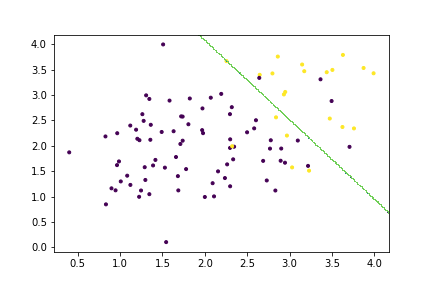
\includegraphics[width=0.8\textwidth]{3b.png}
\end{center}


\question
Minimum value of the objective function is 0 because the cluster centers would be on top of the points themselves, so all cluster distances to each center would be 0.

Optimal $\mu_k$ for regularised k-means and $k=n$. The regularisation will decrease the mean vector's size by bringing it closer to 0, as if there were $\lambda$ extra points at the origin which were part of each cluster.
\begin{align*}
    0   &=  \dv{\mu_n} (\lambda |\mu_n|^2 + r_{nk} |x_n - \mu_n|^2)   \\
    0   &=  \dv{\mu_n} (\lambda \mu_n^T\mu_n + r_{nk} (x_n - \mu_n)^T(x_n-\mu_n)   )    \\
    0   &=  2\lambda \mu_n^T - 2r_{nk} (x_n - \mu_n)^T \\
    0   &=  \lambda \mu_n^T - r_{nk} x_n^T + r_{nk} \mu_n^T \\
    \mu_n^T &=  \frac{r_{nk} x_n^T}{\lambda + r_{nk}} \\
    \mu_k &=  \boxed{\frac{\sum_n r_{nk} x_k}{\lambda + \sum_n r_{nk}}} \\
\end{align*}


\question
skip

\question
A is positive definite for the following value of a.
\begin{align*}
    z^TAz	&=	\begin{pmatrix}z_1&z_2\end{pmatrix} \begin{pmatrix}9&6\\6&a\end{pmatrix} \begin{pmatrix}z_1\\z_2\end{pmatrix}	\\
    0	&\leq	\begin{pmatrix}9z_1+6z_2&6z_2+az_1\end{pmatrix} \begin{pmatrix}z_1\\z_2\end{pmatrix}	\\
    0	&\leq	9z_1^2 + 6z_1z_2 + 6z_1 z_2 + az_2^2	\\
    0	&\leq	12z_1 + az_2	\\
    a	&\geq	\boxed{-12z_1/z_2}	\\
\end{align*}
Proof that inverse of positive definite matrix is also positive definite. Note that since a positive definite matrix is invertible, it spans $R^n$, and every vector $y$ can be expressed as $y = \pm Bz$ for a unique $z$.
\begin{align*}
    0   &\leq   z^T B z   \\
    0   &\leq   z^T I B z   \\
    0   &\leq   z^T B^T B^{-1} B z   \\
    0   &\leq   (Bz)^T B^{-1} (Bz)   \\
    0   &\leq   \boxed{y^T B^{-1} y }   \\
\end{align*}
Data covariance matrix S is positive semi-definite.
\begin{align*}
    z^T S z	&=	z^T \left( \frac{\Sigma_i (x_i-\mu)(x_i-\mu)^T}{n} \right) z	\\
    z^T S z	&=	\frac{1}{n} \Sigma_i z^T (x_i-\mu)(x_i-\mu)^T z	\\
    z^T S z	&=	\frac{1}{n} \Sigma_i ((x_i-\mu)^T z)^T ((x_i-\mu)^T z)	\\
    z^T S z	&=	\frac{\sum|(x_i-\mu)^T z|^2}{n} \\
\end{align*}
Norm of a vector is always at least 0 so \fbox{$z^TSz \geq 0$}.


\question
skip


\end{document}
